\cleardoublepage

\chapter{Séries temporelles}

\begin{wrapfigure}{r}{3cm}
\Youtube{https://youtu.be/xrdCY4iN40s}
\end{wrapfigure}

Les capteurs virtuels que nous avons programmés jusqu’à présent émettent les données à chaque fois que celles-ci sont mesurées. 
Cela permet au serveur de suivre en temps réel le comportement du système étudié. 
Mais dans certains cas, le temps réel n’est pas nécessaire et il est préférable de limiter le nombre d’émissions, par exemple pour économiser l'énergie du capteur.

Pour ce faire, nous pouvons utiliser un tableau qui va accumuler les valeurs et l’envoyer quand le tableau atteint une certaine taille.


\section{Envoi d'un tableau}

Le programme \pprog{minimal\_humidity1.py}{plido-tp3} accumule les données dans un tableau \texttt{h\_humidity} quand celui-ci atteint 30 éléments (ligne 17), les données sont envoyées au serveur.

\pythonlst{minimal\_humidity1.py}



\begin{termc}[backgroundcolor=\color{palerod}, basicstyle=\ttfamily\small, escapechar=\#]
1 4 [3241]
2 7 [3241, 2945]
3 10 [3241, 2945, 2762]
4 13 [3241, 2945, 2762, 2625]
5 16 [3241, 2945, 2762, 2625, 2480]
6 19 [3241, 2945, 2762, 2625, 2480, 2769]
\end{termc}

Le premier chiffre de la ligne indique le nombre d'éléments et le second la taille dans le codage CBOR. On remarque que l'ajout d'un élément augmente la taille du tableau de 3 octets. Les valeurs correspondant à une mesure d'humidité ne varient pas fortement. Ainsi un tableau de 30 mesures a une taille de 92 octets.

\section{Codage par différence}

On peut optimiser le volume de données transférées en utilisant un codage par delta (i.e. la variation de l'humidité). 
La première valeur du tableau correspond à la valeur mesurée tandis que les suivantes représentent la différence entre la valeur mesurée et la précédente.

\pythonlst[firstline=17,lastline=26,  firstnumber=17]{minimal\_humidity2.py}%[firstline=282,lastline=19, firstnumber=282]

Le programme \pprog{minimal\_humidity2.py}{plido-tp3} gère différemment le remplissage du tableau~:

\begin{itemize}
    \item ligne 14 et 15, si le tableau est vide, le tableau est créé avec la valeur mesurée,
    \item ligne 16 à 22, sinon si le tableau est plein, il est sérialisé en CBOR et envoyé au serveur, puis réinitialisé avec la valeur mesurée,
    \item ligne 23 et 24, sinon la différence entre la précédente valeur et celle mesurée est stockée dans le tableau.
\end{itemize}

       \vspace{1em}

Le listing suivant donne un exemple d'exécution.

\begin{termc}[backgroundcolor=\color{palerod}, basicstyle=\ttfamily\small, escapechar=\#]
1 4 [2521]
2 6 [2521, 79]
3 8 [2521, 79, 224]
4 10 [2521, 79, 224, -40]
5 12 [2521, 79, 224, -40, -112]
6 13 [2521, 79, 224, -40, -112, 1]
7 15 [2521, 79, 224, -40, -112, 1, 130]
8 18 [2521, 79, 224, -40, -112, 1, 130, -288]
9 21 [2521, 79, 224, -40, -112, 1, 130, -288, 299]
\end{termc}

Ceci met en valeur deux souplesses de CBOR :
\begin{itemize}
    \item la taille du tableau est dynamique. Si l’on change le nombre de valeurs à transmettre, le tableau l’indique et l’on n’a pas besoin de modifier le code du récepteur ;
    \item la taille des données dépend de leur valeur. 
    Pour les variations entre -24 et +23, un seul octet sera nécessaire. 
    On le voit sur l’exemple précédent : l’ajout de la valeur '1' dans le tableau fait passer la taille de la représentation CBOR de 12 à 135 octets. Les valeurs entre 256 et +255 sont transmises sur 2 octets ; il est donc possible de cette manière d’optimiser la transmission sans ajouter de contrainte. S’il y avait une brusque variation de l’humidité, la représentation CBOR s’adapterait pour la transmettre.
\end{itemize}

La taille est réduite d"un tiers (environ 66 octets) pour transmettre la même information.

\section{Architecture}

La figure~\vref{fig-client-serveur} représente l'architecture générale du système. Le programme \pprog{minimal\_humidity2.py}{plido-tp3} fournit les séries temporelles. Il reste à définir le programme serveur qui va les traiter et faire appel à un autre service pour les afficher sous forme de graphe. 

       \vspace{1em}


Si l'on suit le flux d'information, le capteur va produire des données au format CBOR pour être compact et le programme serveur va transformer cette information en une structure JSON respectant les spécifications du service d'affichage.

\begin{figure}[tbp]
\centerline{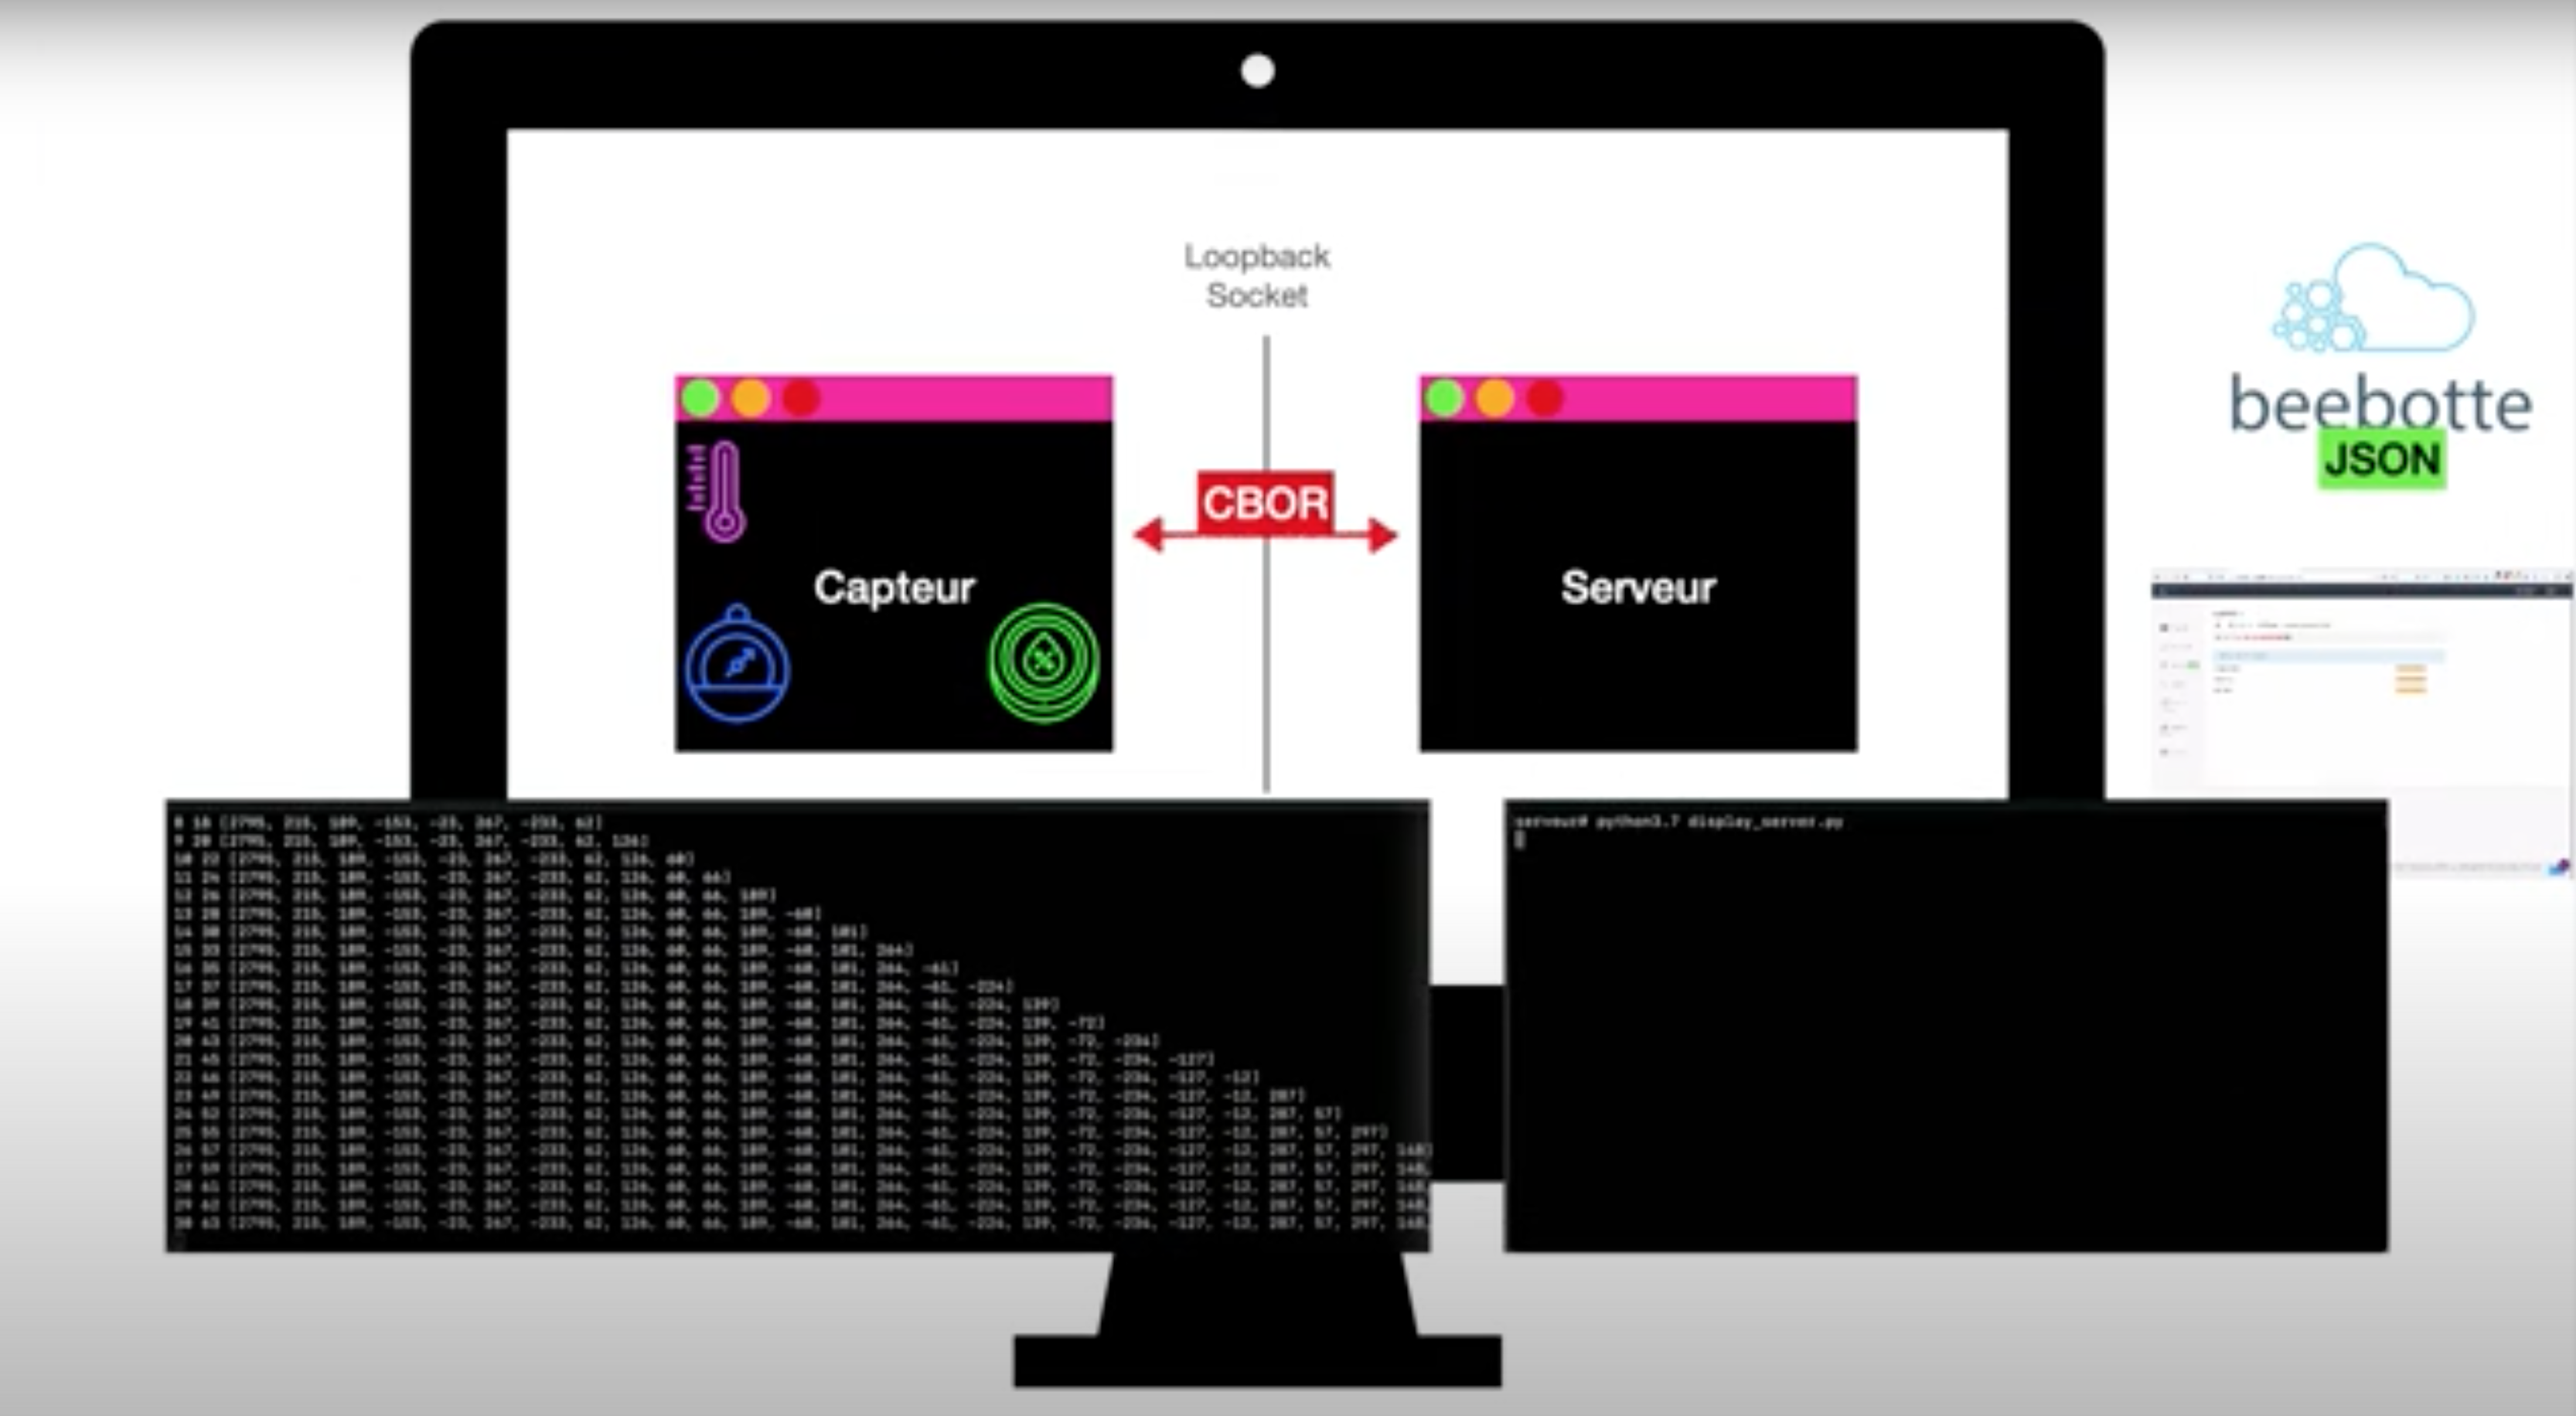
\includegraphics[width=1\columnwidth]{Pictures/Capture40.png}}
\caption{Architecture Client/Serveur}
\label{fig-client-serveur}
\end{figure}

\section{\Index{Beebotte}}

Il existe plusieurs sites qui permettent de le faire. Nous allons utiliser \url{https://beebotte.com}, mais ce que nous allons présenter peut très bien s'appliquer à d'autres sites.

\subsection{Configuration}

\begin{wrapfigure}{r}{3cm}

\includegraphics[width=.2\columnwidth]{Pictures/beebotte.png}
\end{wrapfigure}

La première étape consiste à créer un compte en cliquant sur \textit{Sign Up} sur la page de garde et en remplissant un formulaire classique avec votre login, adresse de courrier électronique et mot de passe. Une fois le compte validé, le service est accessible.

Le compte nous permet de nous authentifier pour gérer les données sur le site, mais il faut également disposer d’autorisation pour pouvoir y déposer des données via l’\Index{API REST}.
Pour cela, il faut se rendre sur la page \textit{Account Setting} puis l’onglet \textit{Access Management}. 
Cette page (cf. figure~\vref{fig-bb-key}) donne une clé et un secret pour gérer l’ensemble des données sur le site. 

\begin{figure}[tbp]
\centerline{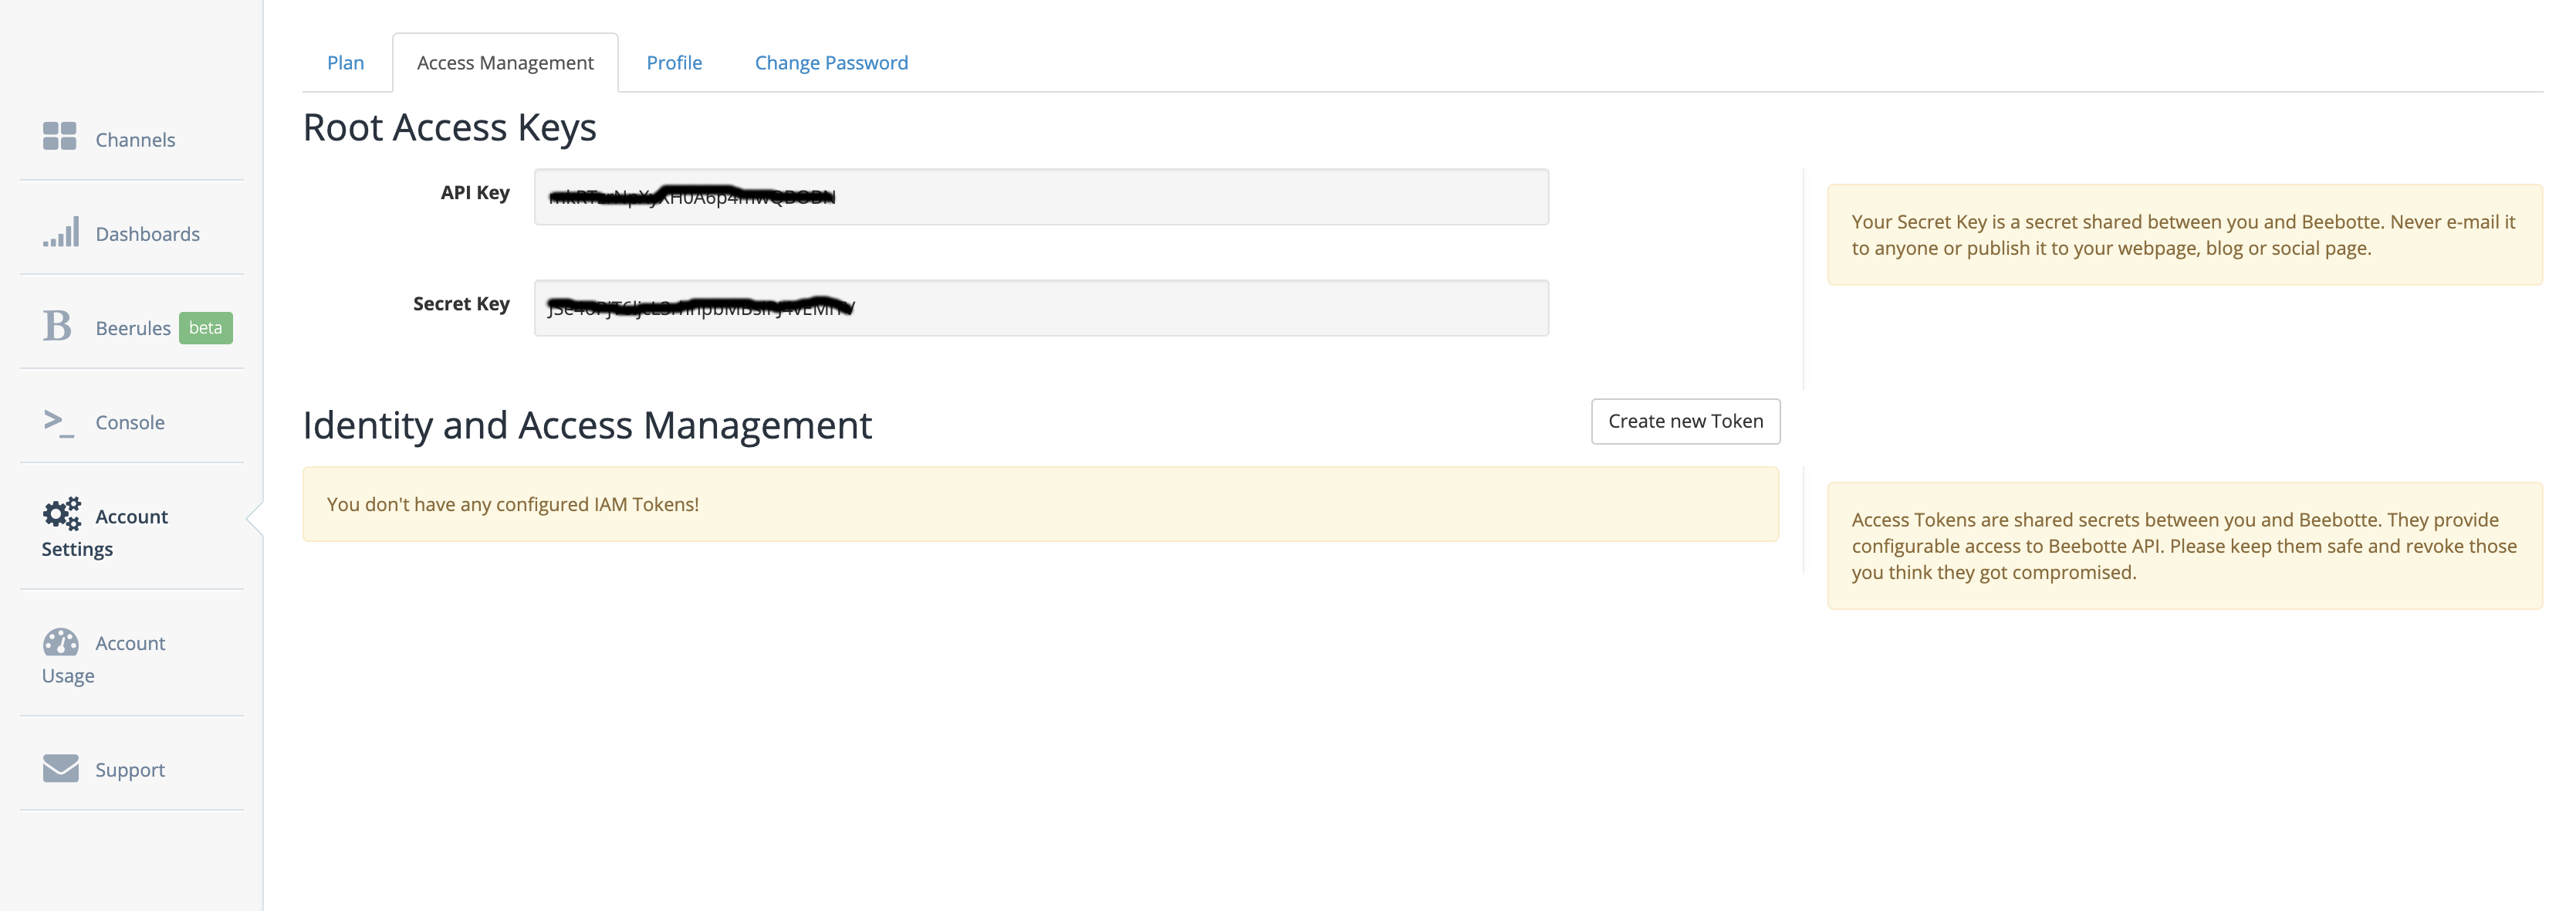
\includegraphics[width=1\columnwidth]{Pictures/bb_root_token.png}}
\caption{Clé et secret pour l'authentification}
\label{fig-bb-key}
\end{figure}


Notez ces valeurs et stockez les dans un fichier \pprog{config\_bbt.py}{plido-tp3} qui a cet aspect (vos valeurs sont forcément différentes) :

\pythonlst{config\_bbt.py}




Nous allons maintenant créer un canal (/textit{channel}) dans lequel nous allons définir les objets correspondant aux capteurs. En Cliquant sur \textit {Channels} puis \textit{Create New}, la page représentée figure~\vref{fig-new-channel} apparaît. 

Il faut donner un nom au channel (\textit{capteurs} dans l'exemple), cocher la case \textit{public} et créer trois ressources pour les trois valeurs qui nous intéressent (\textit{temperature}, \textit{humidity}, \textit{presure}) et faire correspondre les unités.



\subsection{Enregistrement des ressources}

Le programme \pprog{display\_server.py}{plido-tp3} permet de correspondre avec Beebotte via son API REST. Il commence par l'importation des modules nécessaires~:

\pythonlst[firstline=1,lastline=8, firstnumber=1]{display\_server.py}


\begin{itemize}
    \item ligne 4, le module Python \texttt{beebotte}  est disponible pour simplifier la manipulation des données\footnote{S'il n'était pas présent sur votre ordinateur, vous devriez l'installer avec la commande \texttt{pip3 install beebotte}.}.
    \item ligne 5, le module \texttt{contient} la clé et le secret nécessaire à la connexion obtenu précédemment.
    
\end{itemize}



\pythonnxt[firstline=9,lastline=11, firstnumber=9]{display\_server.py}

\begin{itemize}
    \item ligne 10 et 11 permette d'ouvrir la socket pour communiquer avec les capteurs.
\end{itemize}

\pythonnxt[firstline=12,lastline=14, firstnumber=12]{display\_server.py}


\begin{itemize}
    \item ligne 13 une instance permettant la connexion avec les serveurs de Beebotte est définie grâce à la fonction \pfunction{beebotte}{BBT}. Les paramètres de connexion provenant du module \texttt{config\_bbt} sont pris en compte. 
\end{itemize}


\pythonnxt[firstline=41,lastline=45, firstnumber=41]{display\_server.py}

Dans le programme principal, un boucle sans fin attend la série temporelle codée en CBOR venant du capteur (ligne 42), les transforme tableau Python (ligne 44) et appelle la fonction \texttt{to\_btt} en précisant\:
\begin{itemize}
    \item le canal et la ressource qui ont été définie précédemment sur Beebotte~;
    \item la série temporelle
    \item la précision pour transformer ces entiers en flottant.
\end{itemize}
.  

\pythonnxt[firstline=15,lastline=38, firstnumber=15]{display\_server.py}

La fonction \texttt{to\_bbt} fait l’essentiel du travail de transformation. Elle prend en argument :

\begin{itemize}
    \item le nom du canal créé sur Beebotte. Dans notre cas, ce sera \texttt{capteurs} ;
    \item le nom de l’objet dans ce canal que nous avons également créé sur le site web. Dans notre cas, ce sera \texttt{humidity} ;
    \item le tableau python des mesures codées en delta ;
    \item le facteur multiplicatif, c’est-à-dire la précision. Ici, il faudra diviser par 100 ;
    \item la période entre deux mesures ; cela nous permettra de calculer l’instant de la mesure. Par défaut, la période est de 10 secondes ;
    \item le temps de réception du message pour dater les échantillons. S’il n’est pas spécifié, le temps courant est pris.

\end{itemize}

       \vspace{1em}

Cette fonction transforme le tableau Python suivant :
\begin{termc}[backgroundcolor=\color{palerod},  basicstyle=\ttfamily\small, escapechar=\#]
[3311, 124, -144, -188, -94, 289, -1, -72, 1 ...
\end{termc}

en un tableau de dictionnaire :

\begin{termc}[backgroundcolor=\color{palerod},  basicstyle=\ttfamily\small, escapechar=\#]
[{'data': 33.11, 'resource': 'humidity', 'ts': 1596730115000.0},
 {'data': 34.35, 'resource': 'humidity', 'ts': 1596730125000.0},
 {'data': 32.91, 'resource': 'humidity', 'ts': 1596730135000.0},
 {'data': 31.03, 'resource': 'humidity', 'ts': 1596730145000.0},
 ...
\end{termc}

       \vspace{1em}

Chaque dictionnaire contient trois éléments imposés par Beebotte :

\begin{itemize}
\item le nom de la ressource (\texttt{resource}) telle qu'elle a été définie sur l’interface pour le canal ;
\item la valeur associée pour cette ressource (\texttt{data}) ;
\item l’instant à laquelle cette mesure a été faite (\texttt{ts}). Le temps est représenté suivant le format \Index{Epoch} qui compte le nombre de secondes depuis le premier Janvier 1970\footnote{voir \url{https://www.epochconverter.com/} pour les conversions.}.
\end{itemize}

       \vspace{1em}

Le calcul du \textit{timestamp} (\texttt{ts}) est l’opération la plus complexe de cette fonction mais les module \texttt{time} et \texttt{datetime} facilitent le calcul. 
Si l'argument \texttt{epoch} a été fourni lors de l'appel, la fonction prend cette valeur, sinon le calcule ligne 23. La fonction \pfunction{datetime}{now} retourne la date et l'heure courante, qui est transformé en un tuple grâce à la fonction \pfunction{datetime}{timetuple}. A partir de ce dernier, la fonction \pfunction{time}{maketime} le converti en epoch. 



Ligne 25, l'epoch à laquelle la première mesure du tableau a été faite est calculé en prenant le temps actuel (cela suppose que l’on néglige le temps de traitement et de transmission) auquel on retranche la durée de la capture, c’est-à-dire comme le nombre d’éléments du tableau multiplié par l’intervalle entre chaque mesure (\texttt{period}). 

Ligne 32 à 34 la structure attendue par Beebotte est construite. le résultat est envoyé, ligne 38, grâce à la fonction \pfunction{beebotte}{writeBulk} qui permet d'envoyer un ensemble de valeurs dans un tableau.

       \vspace{1em}

On peut vérifier que Beebotte a reçu des données en visualisant le canal capteurs sur l’interface Web. On peut voir sur la  figure~\vref{fig-bb-mesure} que seule la ressource \texttt{humidity} a reçu des données. L’interface affiche la dernière valeur reçue et la date de réception.

\begin{figure}[tbp]
\centerline{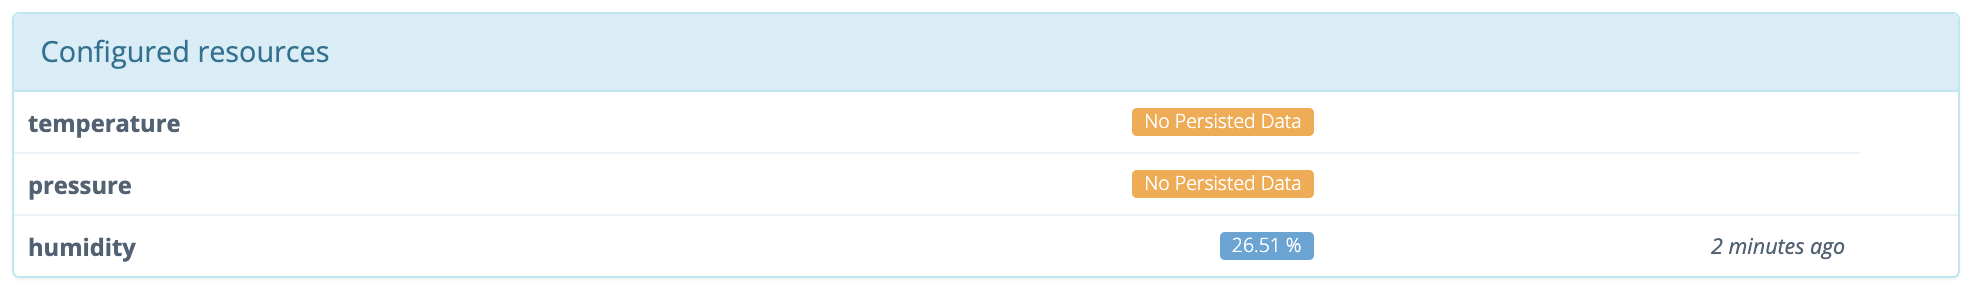
\includegraphics[width=1\columnwidth]{Pictures/bb_mesures.png}}
\caption{État des ressources}
\label{fig-bb-mesure}
\end{figure}

\subsection{Visualisation des ressources}

Maintenant que les ressources sont stockées dans les serveurs de Beebotte, il est possible de les visualiser graphiquement, en allant dans \textit{Dashboard} puis \textit{create Dashboard} et \textit {Add Widget} pour sélectionnez un widget comme \textit{Multi-line chart}.

 

Puis, configurez le widget en définissant le canal et la ressource de ce canal comme le montre la figure~\vref{fig-widget}.

\begin{figure}[tbp]
\centerline{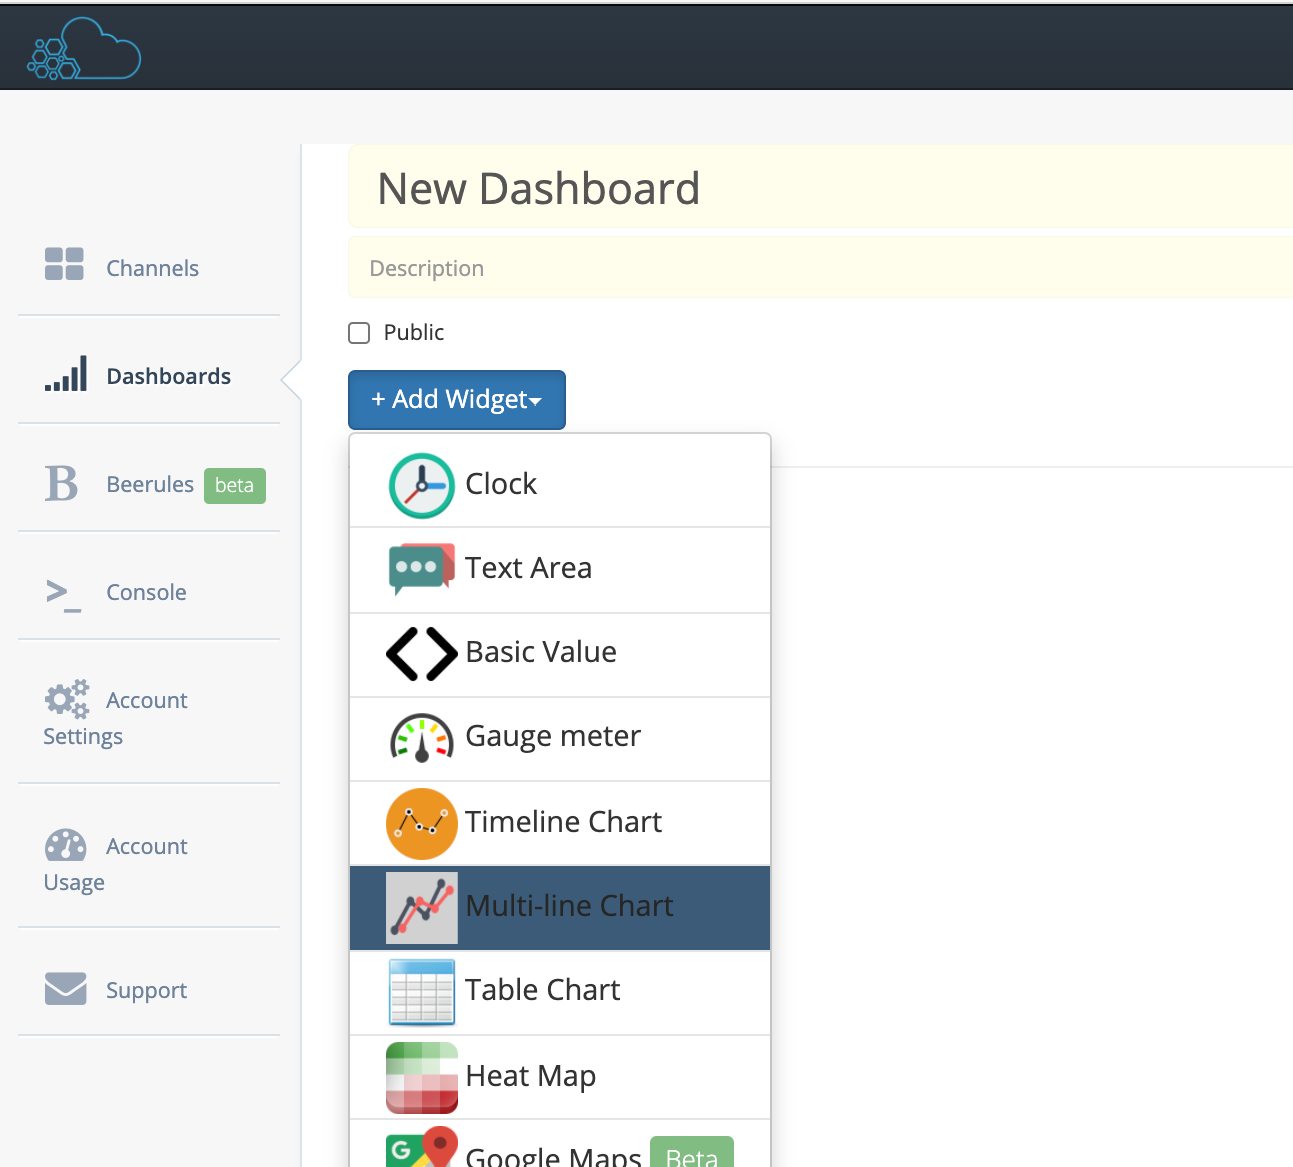
\includegraphics[width=0.5\columnwidth]{Pictures/bb_new_widget.png}}
       \vspace{1em}
\centerline{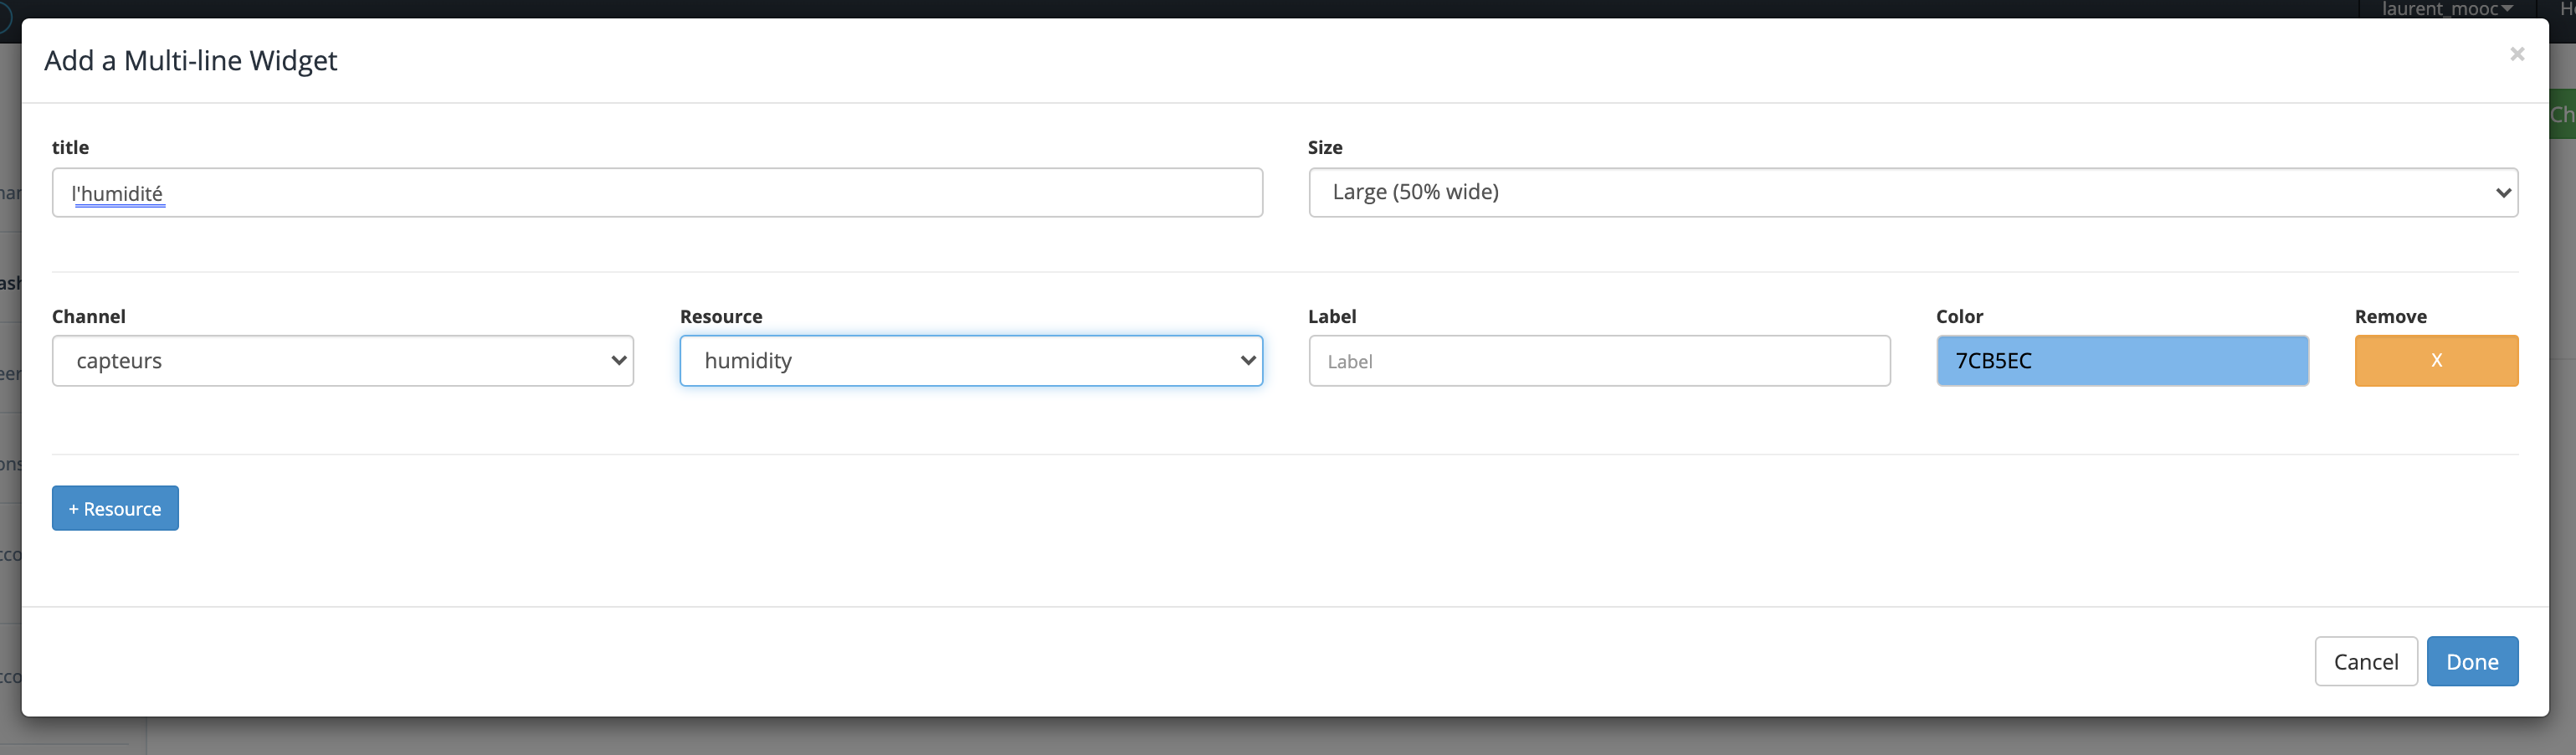
\includegraphics[width=0.5\columnwidth]{Pictures/bb_conf_widget.png}}
\caption{Création d'un widget}
\label{fig-widget}
\end{figure}


En retournant sur le dashboard, on peut voir l’évolution de l’humidité au cours du temps (cf. figure~\vref{fig-bb-humidity}). 

\begin{figure}[tbp]
\centerline{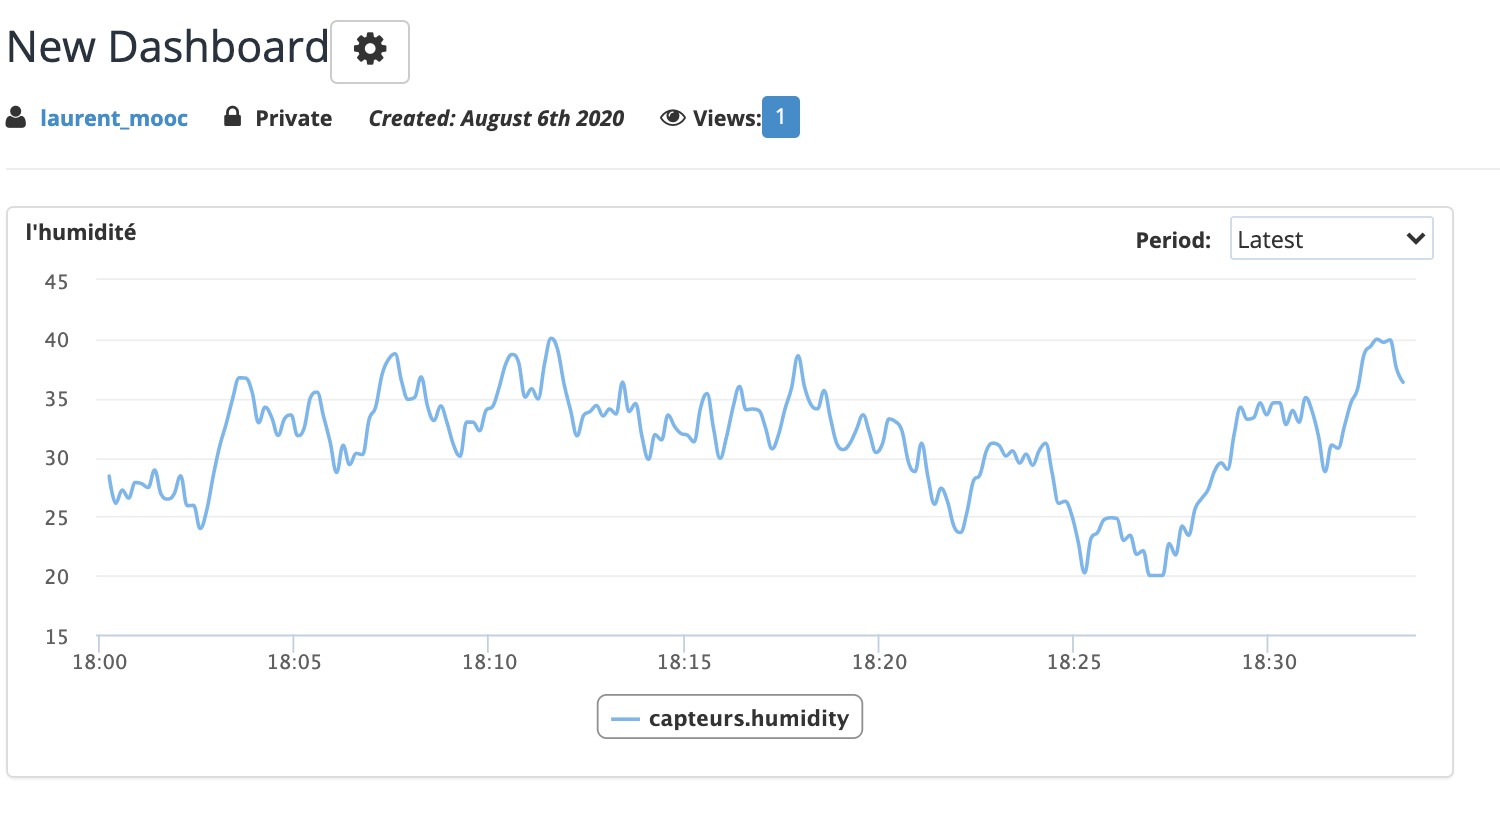
\includegraphics[width=1\columnwidth]{Pictures/bb_humidity.png}}
\caption{Suivi de l'humidité}
\label{fig-bb-humidity}
\end{figure}

\section{Interopérabilité}

La chaîne de collecte de l'information que nous venons de construire allant du capteur à l'affichage, n'est pas complètement interopérable. Certes le capteur envoie des données au format CBOR qui peuvent être interprété par l'autre extrémité, mais le récepteur ne sait pas~:
\begin{itemize}
    \item qu'il s'agit d'une série temporelle codée avec des deltas~;
    \item que les données ont été multipliée par 100 pour pouvoir envoyer des nombres entiers, plus compacts sans perdre trop de précision~;
    \item que le pas de mesure est de 10 secondes
    \item que les données concernent le taux d'humidité.
\end{itemize}

Ces informations ont été précisées dans le programme \pprog{display\_server.py}{plido-tp3}, de même la transformation de la structure de tableau de la série temporelle en un dictionnaire avec des mots clés spécifique à Beebotte on été gravé dans le programme. 

       \vspace{1em}

Nous verrons par la suite comment améliorer cette interopérabilité.

\section{et SenML ?}

Dans la communication avec Beebotte,  le site structure l’envoi des mesures en définissant un dictionnaire JSON avec des mots clés particuliers. Pour utiliser un autre site, le format des échanges doit êter modifié même si les informations restent identiques.

       \vspace{1em}

De plus, lors de la configuration des ressources sur le site de Beebotte, la nature de la mesure a du être précisée~; par exemple, s’il s’agit d’une température, d’un taux d’humidité... Il faut également parfois indiquer le type de la mesure (texte, entier, flottant...) voire les unités. 

       \vspace{1em}

\ac{SenML} défini dans le \rfc{8428} propose une structuration des données fournie par le capteur. 
Pour réduire l’impact de la transmission, les noms des champs ont été choisis pour être le plus compact possible. 
Par exemple, la lettre \texttt{v}  va indiquer une valeur (à comparer avec la clé \texttt{data} utilisée lors de la communication avec Beebotte). 
Pour être encore plus compact, la représentation en CBOR utilisera des entiers courts au lieu de caractères.

       \vspace{1em}

Il est également possible de transporter l’unité de la mesure avec le mot clé \texttt{u} .


SenML ne définit pas que des unités  du système international, mais également des unités secondaires pour limiter la taille de la représentation. Il sera plus compact de transmettre :

\begin{termc}[backgroundcolor=\color{palerod}, basicstyle=\ttfamily\small, escapechar=\#]
{"u": "MHz", "v": 868}
\end{termc}

que
\begin{termc}[backgroundcolor=\color{palerod},  basicstyle=\ttfamily\small, escapechar=\#]
{"u": Hz", "v": 868000000}.
\end{termc}

Le standard définit aussi des temps de base et des valeurs de base auxquelles les temps et les valeurs vont se référer ; ce qui permet également de réduire la taille des valeurs. Finalement, le ou les objets peuvent s’identifier dans les données transmises en définissant un nom de base (\texttt{bn} : \textit{base name}), le nom du capteur (\texttt{n} : \textit{name}) vient compléter le nom de base.

\subsubsection{Émission}

\pythonlst{minimal\_senml\_client.py}

Le programme \pprog{minimal\_senml\_client.py}{plido-tp3} illustre le fonctionnement de SenML. Il repose sur deux objets~:
\begin{itemize}
\item l'objet \pfunction{kpn\_senml}{SenmlPack} inclus les informations commune à l'objet, comme le nom de base (ici \texttt{device1} ligne 23) ou la base de temps, ligne 24.
\item l'objet \pfunction{kpn\_senml}{SenmlRecord} contient une mesure où l'on peut préciser son nom, son unité et sa valeur (lignes 32, 38 et 43). Le temps est également précisé ligne 35. Ces enregistrements sont ajoutés à l'objet \texttt{pack}.
\end{itemize}

Le programme récupère les trois valeurs de température, humidité et pression (lignes 27 à 29) en les arrondissant à 2 chiffres après la virgule pour la température et l'humidité et converti la pression, d'hecto Pascal en Pascal puisque c'est l'unité définie par SenML. 

Les mesures se font toutes les 10 seconde (délais ligne 48) et quand le nombre de mesures défini ligne 13 est atteint, le codage SenML en CBOR est envoyé au serveur. 

       \vspace{1em}

\begin{termc}[backgroundcolor=\color{palerod}, basicstyle=\ttfamily\small, escapechar=\#]
[{'bn': 'device1', 'bt': 1640110457.0,  
  'n': 'temperature', 't': 0.0, 'u': 'Cel',   'v': 19.98},
 {'n': 'humidity', 'u': '%RH', 'v': 28.46},
 {'n': 'pressure', 'u': 'Pa', 'v': 100093}]
JSON length:  177 bytes
CBOR length:  104 bytes
\end{termc}

Ce premier listing montre le premier enregistrement pour les trois grandeurs mesurées. Il s'agit d'un tableau de 3 éléments. Le premier contient les valeurs de bases (ici le nom et l'heure de référence) suivi de la grandeur à mesurer, de son unité et sa valeur. Le deuxième et le troisième éléments, mettent à jours le nom de la grandeur, son unité et sa valeur, les autres informations précédemment définies restent valables.


\begin{termc}[backgroundcolor=\color{palerod},  basicstyle=\ttfamily\small, escapechar=@]
[@\textcolor{gray}{\{'bn': 'device1',  'bt': 1640110457.0,}@
 @\textcolor{gray}{ 'n': 'temperature',  't': 0.0, 'u': 'Cel', 'v': 19.98\},}@
 @\textcolor{gray}{\{'n': 'humidity', 'u': '\%RH', 'v': 28.46\},}@
 @\textcolor{gray}{\{'n': 'pressure', 'u': 'Pa', 'v': 100093\},}@
 {'n': 'temperature', 't': 10.0, 'u': 'Cel', 'v': 20.03},
 {'n': 'humidity', 'u': '%RH', 'v': 26.86},
 {'n': 'pressure', 'u': 'Pa', 'v': 100065}]
JSON length:  318 bytes
CBOR length:  188 bytes
 \end{termc}
 
 Quand on ajoute 10 secondes plus tard de nouvelles mesures,  un temps relatif de 10 secondes est indiqué pour l'enregistrement des températures et il reste valable pour les enregistrements suivants.
 
 \Question{codage}
 {A quoi correspond la clé \texttt{'u' : 'Cel'} que l'on retrouve dans la structure précédente ? }
 {Unité = degrés Celcius}
 
 \Question{Accroissement}
 {Dans les deux représentations JSON et CBOR, de combien la taille est-elle accrue par l'ajout des mesures effectuées ? d'où viennent ces différences ?}
 {
 Si l'on regarde le listing précédent, l'ajout des trois mesures fait augmenter la taille de 141 octets pour JSON et 84 pour CBOR. La différence vient de l'utilisation de nombre plus que de chaînes de caractères pour les clés. Ainsi 't' demande 3 caractères en JSON avec les guillemets, codé en CBOR, il faudrait 2 octets, un nombre inférieur à 23 se code sur un seul octet. Il y a egalement les virgules, espaces et fermeture de crochets qui ne sont pas présent en CBOR. Les nombres flottant comme \texttt{19.98} ont une représentation plus compacte en JSON (5 octets) qu'en CBOR où ils consomment 9 octets. Dans tous les cas l'accroissement est fortement dépendant du nom des éléments. Ici, il faut répéter à chaque fois \texttt{temperature}, \texttt{humidity} et \texttt{pressure}, soit 26 caractères.
 }
 
 \Question {Une seule grandeur}
 {Si on ne s'intéressait qu'à une seule grandeur, par exemple l'humidité. A quoi ressemblerait la structure SenML en JSON ?}
 {
 Chaque nouvelle entrée ajoute 35 octets à la structure~: 
 [\{'bn': 'device1',  'bt': 1640110457.0, 'n': 'humidty', 'u': '\%RH', 'v': 28.46\},\\
 \{'t': 10.0, 'v': 26.86\},\\
 \{'t': 20.0, 'v': 26.96\},\\
 \{'t': 30.0, 'v': 27.01\}]\\
 }
 
 \subsubsection{Réception}
 
 Le traitement par le module SenML tel qu'il est mis en œuvre n'est pas complet, il ne gère pas correctement les timestamps. Mais, il n'est pas vraiment nécessaire pour traiter ces messages. En effet, comme on l'a vu précédemment, les objets SenML sont cumulatifs, une clé reste présente dans les enregistrements suivants sauf si elle est redéfinie. 
 
 
 \pythonlst{minimal\_senml\_server.py}
 
 Le programme \pprog{minimal\_senml\_server.py}{plido-tp3} va convertir le format SenML codé en CBOR dans le format attendu par Beebotte. 
 La version CBOR utilise ds nombres plutôt que des tags.
 Le dictionnaire \texttt{naming\_map} defini lignes 10 à 12 permet la correspondance utilisé par la suite pour rendre le code plus lisible.
 
 Les lignes 14 à 17 initialisent les communications venant du capteur et celles allant à Beebotte. 
 
 Les données reçues ligne 21 sont transformée en structure Python ligne 23. Cette correspondance est possible car Python autorise des clés numériques et celles-ci ne sont pas répétées plusieurs fois dans une map CBOR.
 
La boucle commençant ligne 28 permet d'explorer tous les éléments du tableau SenML, les nouvelles entrées sont fusionnées avec les anciennes (ligne 29)\footnote{Dans les version plus récentes de Python, il est possible d'utiliser l'opérateur \texttt{|}.}. 

Les informations concernant le temps sont ensuite recherchées. 
D'abord le temps (ligne 32) et s'il un temps de base existe (ligne 33) il est ajouté. On procède de même pour la valeur (lignes 38 à 40). Pour le nom, il n'y a pas de concaténation car le nom de base sera utilisé comme canal Beebotte, il est récupéré à la fin ligne 46.

A partir de ces informations, la structure attendue par Beebotte est construite ligne 43 en ajoutant le dictionnaire dans le tableau \texttt{bbt\_record}.

Ligne 47, l'information est envoyée à Beebotte. Si les clés d'authentification, le nom du canal et des ressources sont correct, les information s'affiche sur le site, comme précédemment. 

\begin{termc}[backgroundcolor=\color{palerod},  basicstyle=\ttfamily\tiny, escapechar=@]
{0: 'temperature', 1: 'Cel', 2: 19.44, 6: 0.0, -3: 1640168049.0, -2: 'device1'}
{0: 'humidity', 1: '%RH', 2: 24.13, 6: 0.0, -3: 1640168049.0, -2: 'device1'}
{0: 'pressure', 1: 'Pa', 2: 101080, 6: 0.0, -3: 1640168049.0, -2: 'device1'}
{0: 'temperature', 1: 'Cel', 2: 19.48, 6: 10.0, -3: 1640168049.0, -2: 'device1'}
{0: 'humidity', 1: '%RH', 2: 21.85, 6: 10.0, -3: 1640168049.0, -2: 'device1'}
{0: 'pressure', 1: 'Pa', 2: 101090, 6: 10.0, -3: 1640168049.0, -2: 'device1'}
{0: 'temperature', 1: 'Cel', 2: 19.57, 6: 20.0, -3: 1640168049.0, -2: 'device1'}
{0: 'humidity', 1: '%RH', 2: 21.09, 6: 20.0, -3: 1640168049.0, -2: 'device1'}
{0: 'pressure', 1: 'Pa', 2: 101058, 6: 20.0, -3: 1640168049.0, -2: 'device1'}
{0: 'temperature', 1: 'Cel', 2: 19.52, 6: 30.0, -3: 1640168049.0, -2: 'device1'}
{0: 'humidity', 1: '%RH', 2: 20.39, 6: 30.0, -3: 1640168049.0, -2: 'device1'}
{0: 'pressure', 1: 'Pa', 2: 101120, 6: 30.0, -3: 1640168049.0, -2: 'device1'}
{0: 'temperature', 1: 'Cel', 2: 19.44, 6: 40.0, -3: 1640168049.0, -2: 'device1'}
{0: 'humidity', 1: '%RH', 2: 21.94, 6: 40.0, -3: 1640168049.0, -2: 'device1'}
{0: 'pressure', 1: 'Pa', 2: 101128, 6: 40.0, -3: 1640168049.0, -2: 'device1'}
[{'data': 19.44, 'resource': 'temperature', 'ts': 1640168049000.0},
 {'data': 24.13, 'resource': 'humidity', 'ts': 1640168049000.0},
 {'data': 101080, 'resource': 'pressure', 'ts': 1640168049000.0},
 {'data': 19.48, 'resource': 'temperature', 'ts': 1640168059000.0},
 {'data': 21.85, 'resource': 'humidity', 'ts': 1640168059000.0},
 {'data': 101090, 'resource': 'pressure', 'ts': 1640168059000.0},
 {'data': 19.57, 'resource': 'temperature', 'ts': 1640168069000.0},
 {'data': 21.09, 'resource': 'humidity', 'ts': 1640168069000.0},
 {'data': 101058, 'resource': 'pressure', 'ts': 1640168069000.0},
 {'data': 19.52, 'resource': 'temperature', 'ts': 1640168079000.0},
 {'data': 20.39, 'resource': 'humidity', 'ts': 1640168079000.0},
 {'data': 101120, 'resource': 'pressure', 'ts': 1640168079000.0},
 {'data': 19.44, 'resource': 'temperature', 'ts': 1640168089000.0},
 {'data': 21.94, 'resource': 'humidity', 'ts': 1640168089000.0},
 {'data': 101128, 'resource': 'pressure', 'ts': 1640168089000.0}]
 \end{termc}
 
 Le listing précédent montre cette transformation.
 Les premières lignes correspondent aux enregistrements fusionnées et le tableau final, ce qui a été envoyé à Beebotte.
 
 \Question{base value}
 {
 Pourrait-on utiliser le champ SenML \textit{base value} pour diminuer la taille des données de pression atmosphérique~?
 }
 {
Cela serait possible, si cette ressource était envoyée seule.
 }